\chapter{Besoins fonctionnels}

\section{Modèle}
\subsection{Besoins}
Il décrit les données manipulées par l'application. Dans un premier temps, notre modèle est celui des créatures, par la suite, nous utiliserons un modèle basé sur la bourse.
Priorité: importante.
Justification: représente une base de notre application, l'algorithme génétique va être appliqué à ce modèle.


\subsection{Prototype papier}

\begin{figure}[H]
    \centering
    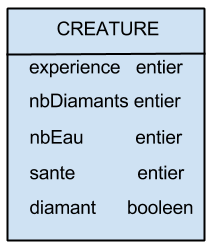
\includegraphics[width=0.3\textwidth]{./pictures/creature.png}
    \caption{Modèle de Creature}
\end{figure}



\section{Réseau de neurones}
\subsection{Besoins}
Permet à notre modèle de définir des actions en fonction des entrées(capteurs, etc). Il s'adapte suivant le modèle, c'est a dire au nombre et au type d'entrées.
Priorité: importante.
Justification: c'est le cerveau du modèle, il est adapté au fil des générations.
\subsection{Prototype papier}

\begin{figure}[H]
    \centering
    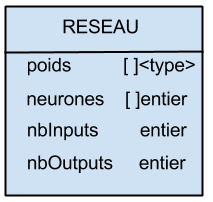
\includegraphics[width=0.3\textwidth]{./pictures/reseau.png}
    \caption{Réseau de neurones}
\end{figure}

\section{Algorithme génétique}
\subsection{Besoins}
Cela représente le type d'algorithme utilisé par notre application, il reste le même quel que soit le modèle.
Priorité: très importante.
Justification: c'est ce qui nous permettre de faire évoluer le modèle durant plusieurs génération jusqu'à obtenir une solution, tendant vers l'optimale.
\subsection{Prototype papier}

\begin{figure}[H]
    \centering
    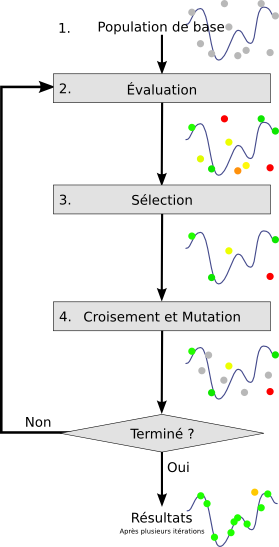
\includegraphics[width=0.4\textwidth]{./pictures/algorithme_genetique.png}
    \caption{Algorithme génétique}
\end{figure}


\section{Interface graphique}
\subsection{Besoins}
Description: nous avons besoin d'une méthode de visualisation clair et pertinente, de nos résultats.
Priorité: importante.
Justification: Afin d’avoir un résultat visuel nous avons besoin d’une interface qui va nous 
montrer en temps réel les agissement des créatures ainsi que leur évolution.

\subsection{Prototype papier}
\begin{figure}[H]
    \centering
    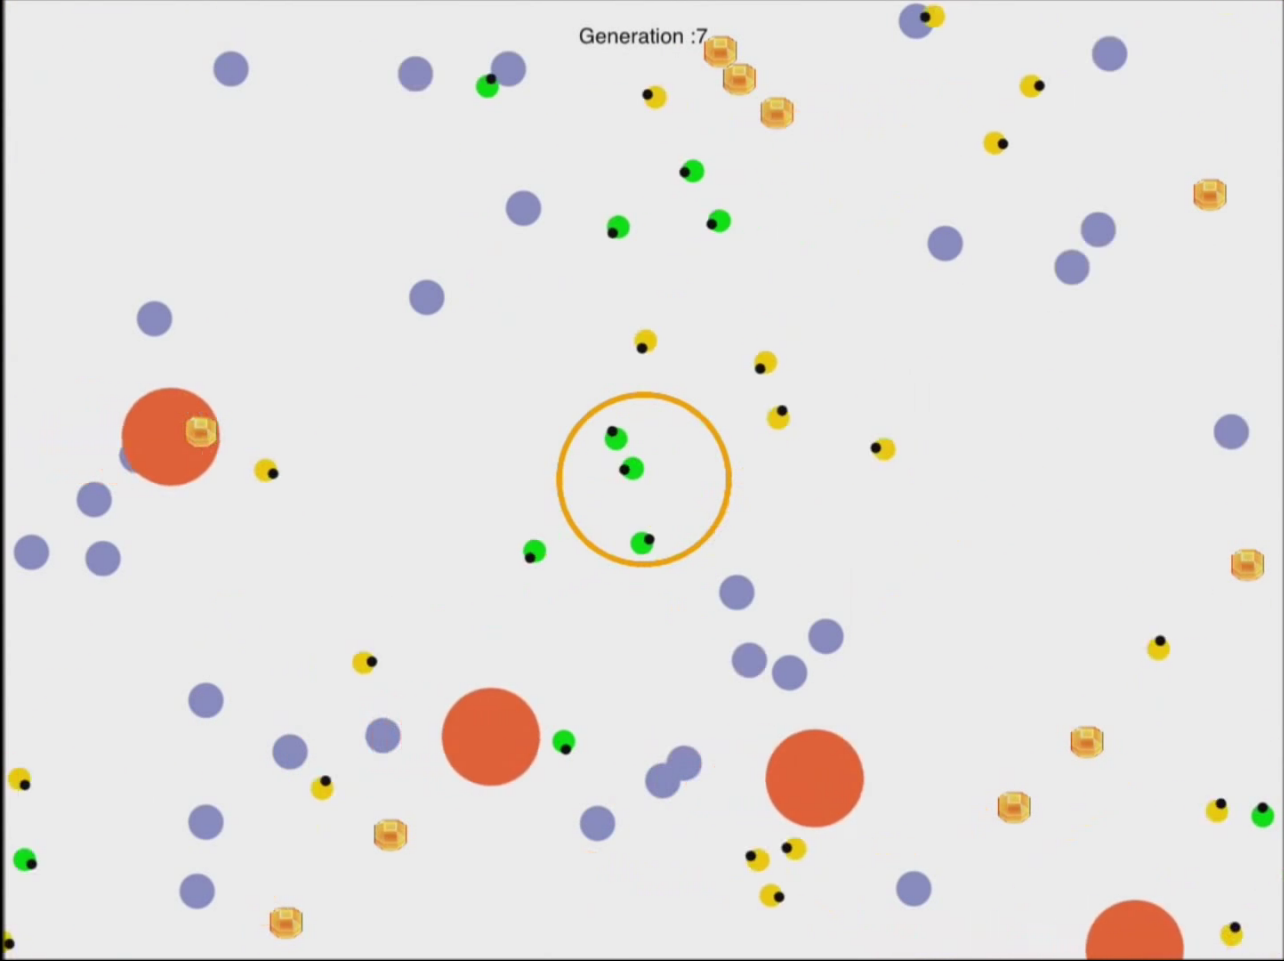
\includegraphics[width=0.8\textwidth]{./pictures/prototype.png}
    \caption{Interface}
    \label{fig:awesome_image}
\end{figure}


\clearpage
